\documentclass[tikz,border=12pt]{standalone}
\usepackage[T1]{fontenc}
\usepackage{mathpazo}
\usepackage{amsmath,amssymb}
\usetikzlibrary{arrows.meta, calc}

\definecolor{stblue}{HTML}{7B97AD}
\definecolor{rwgold}{HTML}{B8995E}
\definecolor{sage}{HTML}{7A9A7E}
\definecolor{dkbrown}{HTML}{3D3530}
\definecolor{wmgray}{HTML}{7B7067}
\definecolor{cream}{HTML}{F9F6F0}
\definecolor{border}{HTML}{D4C9B8}
\definecolor{terracotta}{HTML}{C47A6A}
\definecolor{lavender}{HTML}{907EA0}

\begin{document}
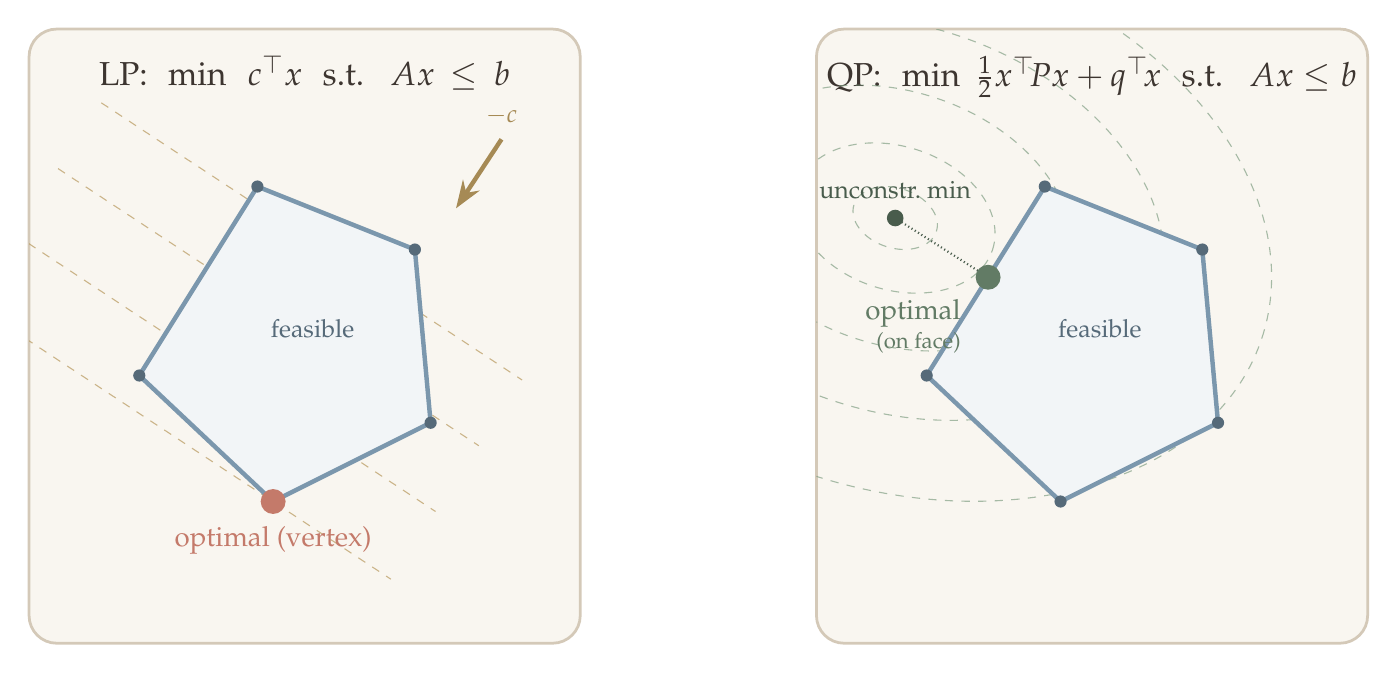
\begin{tikzpicture}[
  >={Stealth[length=3.5mm, width=2.5mm]},
  line width=1.2pt
]

% ============================================================
%  Shared polygon vertices (pentagon), centroid roughly at (0.9, 0.16)
%  Vertices: A=(0.3,2.2), B=(2.3,1.4), C=(2.5,-0.8), D=(0.5,-1.8), E=(-1.2,-0.2)
% ============================================================
\newcommand{\polypath}{
  (0.3, 2.2) -- (2.3, 1.4) -- (2.5, -0.8) -- (0.5, -1.8) -- (-1.2, -0.2) -- cycle
}

% ============================================================
%  LEFT PANEL: LP
% ============================================================
\begin{scope}[shift={(-5.0,0)}]

% Background card
\fill[cream, rounded corners=10pt] (-2.6,-3.6) rectangle (4.4,4.2);
\draw[border, line width=1pt, rounded corners=10pt] (-2.6,-3.6) rectangle (4.4,4.2);

% Title
\node[dkbrown, font=\large, anchor=north, text width=6.4cm, align=center]
  at (0.9, 4.0) {LP:\; $\min\; c^\top x$\; s.t.\; $Ax \leq b$};

% ── Level sets of c^T x (drawn first, behind polygon) ──
% c = (0.55, 0.835), |c|^2 = 0.3025 + 0.697225 = 0.999725 ≈ 1
% Level-set direction (tangent): (-0.835, 0.55)
% Optimal vertex D = (0.5, -1.8): c^T D = 0.275 - 1.503 = -1.228
% We draw 4 level sets from near-optimal up through the feasible region
\begin{scope}
  \clip[rounded corners=10pt] (-2.6,-3.6) rectangle (4.4,4.2);
  \foreach \val in {-1.23, -0.2, 0.8, 1.8}{
    \pgfmathsetmacro{\cx}{0.55*\val}
    \pgfmathsetmacro{\cy}{0.835*\val}
    \draw[rwgold, dashed, thin, opacity=0.7]
      ({\cx - 3.2*0.835}, {\cy + 3.2*0.55})
      -- ({\cx + 3.2*0.835}, {\cy - 3.2*0.55});
  }
\end{scope}

% Feasible polygon
\fill[stblue!10] \polypath;
\draw[stblue, thick, line width=1.6pt] \polypath;

% Polygon vertices
\foreach \p in {(0.3,2.2),(2.3,1.4),(2.5,-0.8),(0.5,-1.8),(-1.2,-0.2)}{
  \fill[stblue!70!black] \p circle (2.2pt);
}

% Feasible region label
\node[stblue!70!black, font=\small] at (1.0, 0.4) {feasible};

% Arrow showing direction -c (direction of decrease)
\draw[->, rwgold!90!black, line width=1.6pt]
  (3.4, 2.8) -- ({3.4 - 1.05*0.55}, {2.8 - 1.05*0.835});
\node[rwgold!90!black, font=\small, anchor=south] at (3.4, 2.85) {$-c$};

% Optimal point at vertex D = (0.5, -1.8)
\fill[terracotta] (0.5, -1.8) circle (4.5pt);
\node[terracotta, font=\normalsize, anchor=north, yshift=-5pt]
  at (0.5, -1.8) {optimal (vertex)};

\end{scope}

% ============================================================
%  RIGHT PANEL: QP
% ============================================================
\begin{scope}[shift={(5.0,0)}]

% Background card
\fill[cream, rounded corners=10pt] (-2.6,-3.6) rectangle (4.4,4.2);
\draw[border, line width=1pt, rounded corners=10pt] (-2.6,-3.6) rectangle (4.4,4.2);

% Title
\node[dkbrown, font=\large, anchor=north, text width=6.8cm, align=center]
  at (0.9, 4.0) {QP:\; $\min\; \tfrac{1}{2}x^\top\! Px + q^\top\! x$\; s.t.\; $Ax \leq b$};

% ── Unconstrained minimizer (outside the polyhedron, to the left) ──
% Place it to the left of the edge E--A, which runs from (-1.2,-0.2) to (0.3,2.2)
\coordinate (qstar) at (-1.6, 1.8);

% ── Elliptical contour lines (drawn first, behind polygon) ──
\begin{scope}
  \clip[rounded corners=10pt] (-2.6,-3.6) rectangle (4.4,4.2);
  \begin{scope}[shift={(qstar)}, rotate=-18]
    \draw[sage, dashed, thin, opacity=0.65] (0,0) ellipse (0.55 and 0.38);
    \draw[sage, dashed, thin, opacity=0.65] (0,0) ellipse (1.3 and 0.91);
    \draw[sage, dashed, thin, opacity=0.65] (0,0) ellipse (2.3 and 1.61);
    \draw[sage, dashed, thin, opacity=0.65] (0,0) ellipse (3.5 and 2.45);
    \draw[sage, dashed, thin, opacity=0.65] (0,0) ellipse (4.9 and 3.43);
  \end{scope}
\end{scope}

% Feasible polygon (same as LP)
\fill[stblue!10] \polypath;
\draw[stblue, thick, line width=1.6pt] \polypath;

% Polygon vertices
\foreach \p in {(0.3,2.2),(2.3,1.4),(2.5,-0.8),(0.5,-1.8),(-1.2,-0.2)}{
  \fill[stblue!70!black] \p circle (2.2pt);
}

% Feasible region label
\node[stblue!70!black, font=\small] at (1.0, 0.4) {feasible};

% Mark unconstrained minimizer
\fill[sage!60!black] (qstar) circle (3pt);
\node[sage!60!black, font=\small, anchor=south, yshift=3pt]
  at (qstar) {unconstr.\ min};

% ── Optimal point on edge E--A ──
% Edge from E=(-1.2,-0.2) to A=(0.3,2.2): direction (1.5, 2.4)
% Project qstar=(-1.6,1.8) onto this edge:
% t = [(-1.6-(-1.2))*1.5 + (1.8-(-0.2))*2.4] / (1.5^2+2.4^2)
%   = [(-0.4)*1.5 + 2.0*2.4] / (2.25+5.76) = [-0.6+4.8]/8.01 = 4.2/8.01 ≈ 0.524
\pgfmathsetmacro{\topt}{0.52}
\coordinate (qopt) at ({-1.2+1.5*\topt}, {-0.2+2.4*\topt});

% Dashed line from unconstrained min to optimal on face
\draw[sage!60!black, thin, densely dotted, line width=0.8pt] (qstar) -- (qopt);

\fill[sage!80!black] (qopt) circle (4.5pt);
\node[sage!80!black, font=\normalsize, anchor=north east, xshift=-6pt, yshift=-4pt]
  at (qopt) {\shortstack[r]{optimal\\[-1pt]{\footnotesize(on face)}}};

\end{scope}

\end{tikzpicture}
\end{document}
